% AUTO-GENERATED by paper/analysis/generate_tables.py -- do not hand-edit.
% Source: evaluation/ground_truth_detector/KY.json, task2_20260826/review_detector/KY/, task3_20260826/review_detector_off/KY/
% Regenerate with: python paper/analysis/generate_tables.py
% Corpus tier (guardrail 1): every row is the _only_subset tier, never full-document.
\begin{figure}[t]
\centering
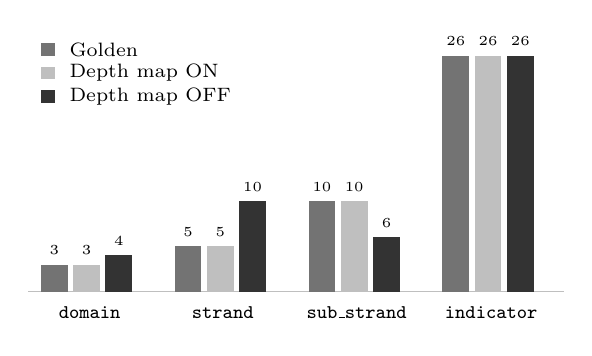
\begin{tikzpicture}[x=1cm, y=1cm]
\draw[gray!50] (0,0) -- (6.80,0);
\fill[black!55] (0.16,0) rectangle (0.50,0.346);
\node[font=\tiny, anchor=south] at (0.33,0.346) {3};
\fill[black!25] (0.57,0) rectangle (0.91,0.346);
\node[font=\tiny, anchor=south] at (0.74,0.346) {3};
\fill[black!80] (0.98,0) rectangle (1.32,0.462);
\node[font=\tiny, anchor=south] at (1.15,0.462) {4};
\node[font=\scriptsize, anchor=north] at (0.78,-0.06) {\texttt{domain}};
\fill[black!55] (1.86,0) rectangle (2.20,0.577);
\node[font=\tiny, anchor=south] at (2.03,0.577) {5};
\fill[black!25] (2.27,0) rectangle (2.61,0.577);
\node[font=\tiny, anchor=south] at (2.44,0.577) {5};
\fill[black!80] (2.68,0) rectangle (3.02,1.154);
\node[font=\tiny, anchor=south] at (2.85,1.154) {10};
\node[font=\scriptsize, anchor=north] at (2.47,-0.06) {\texttt{strand}};
\fill[black!55] (3.56,0) rectangle (3.90,1.154);
\node[font=\tiny, anchor=south] at (3.73,1.154) {10};
\fill[black!25] (3.97,0) rectangle (4.31,1.154);
\node[font=\tiny, anchor=south] at (4.14,1.154) {10};
\fill[black!80] (4.38,0) rectangle (4.72,0.692);
\node[font=\tiny, anchor=south] at (4.55,0.692) {6};
\node[font=\scriptsize, anchor=north] at (4.17,-0.06) {\texttt{sub\_strand}};
\fill[black!55] (5.26,0) rectangle (5.60,3.000);
\node[font=\tiny, anchor=south] at (5.43,3.000) {26};
\fill[black!25] (5.67,0) rectangle (6.01,3.000);
\node[font=\tiny, anchor=south] at (5.84,3.000) {26};
\fill[black!80] (6.08,0) rectangle (6.42,3.000);
\node[font=\tiny, anchor=south] at (6.25,3.000) {26};
\node[font=\scriptsize, anchor=north] at (5.88,-0.06) {\texttt{indicator}};
\fill[black!55] (0.16,3.00) rectangle (0.34,3.16);
\node[font=\scriptsize, anchor=west] at (0.40,3.08) {Golden};
\fill[black!25] (0.16,2.70) rectangle (0.34,2.86);
\node[font=\scriptsize, anchor=west] at (0.40,2.78) {Depth map ON};
\fill[black!80] (0.16,2.40) rectangle (0.34,2.56);
\node[font=\scriptsize, anchor=west] at (0.40,2.48) {Depth map OFF};
\end{tikzpicture}
\caption{Elements emitted per hierarchy level on Kentucky, whose detector golden is the corpus's only \emph{detection-exhaustive} one, with the depth-map pass enabled and ablated. With the pass enabled the detector reproduces the golden distribution exactly. Ablated, it emits an extra domain, doubles the strand count and loses four sub-strands, while the indicator count is untouched --- the failure is level \emph{collapse} at the two levels whose identity is positional rather than typographic. \textbf{This is not visible in a level-confusion matrix}: the evaluation matcher pairs on level, so an element emitted at the wrong level is recorded as a miss rather than an off-diagonal entry, and both arms render as clean diagonals. \texttt{\_only\_subset} corpus tier.}
\label{fig:levels}
\end{figure}
